%% 
%% Copyright 2007, 2008, 2009 Elsevier Ltd
%% 
%% This file is part of the 'Elsarticle Bundle'.
%% ---------------------------------------------
%% 
%% It may be distributed under the conditions of the LaTeX Project Public
%% License, either version 1.2 of this license or (at your option) any
%% later version.  The latest version of this license is in
%%    http://www.latex-project.org/lppl.txt
%% and version 1.2 or later is part of all distributions of LaTeX
%% version 1999/12/01 or later.
%% 
%% The list of all files belonging to the 'Elsarticle Bundle' is
%% given in the file `manifest.txt'.
%% 

%% Template article for Elsevier's document class `elsarticle'
%% with numbered style bibliographic references
%% SP 2008/03/01
% \documentclass[
% 	fontsize=11pt, % Base font size
% 	twoside=false, % Use different layouts for even and odd pages (in particular, if twoside=true, the margin column will be always on the outside)
% 	open=any, % If twoside=true, uncomment this to force new chapters to start on any page, not only on right (odd) pages
% 	secnumdepth=1, % How deep to number headings. Defaults to 1 (sections)
% ]{kaobook}
% \setchapterstyle{kao} % Choose the default chapter heading style


%% Use the option review to obtain double line spacing
%% \documentclass[authoryear,preprint,review,12pt]{elsarticle}

%% For including figures, graphicx.sty has been loaded in
%% elsarticle.cls. If you prefer to use the old commands
%% please give \usepackage{epsfig}

%% The amssymb package provides various useful mathematical symbols

%%% Highlight revisions in blue
% \newcommand{}[1]{#1}
% \newcommand{}[1]{#1}
% Remove the following line to remove highlights
%\renewcommand{}[1]{\textcolor{blue}{#1}}
%\renewcommand{}[1]{\textcolor{blue}{#1}}

%% The lineno packages adds line numbers. Start line numbering with
%% \begin{linenumbers}, end it with \end{linenumbers}. Or switch it on
%% for the whole article with \linenumbers.
% \usepackage{lineno}

% \journal{Knowledge-Based Systems}

% \begin{document}

% \begin{frontmatter}

%% Title, authors and addresses

%% use the tnoteref command within \title for footnotes;
%% use the tnotetext command for theassociated footnote;
%% use the fnref command within \author or \address for footnotes;
%% use the fntext command for theassociated footnote;
%% use the corref command within \author for corresponding author footnotes;
%% use the cortext command for theassociated footnote;
%% use the ead command for the email address,
%% and the form \ead[url] for the home page:
%% \title{Title\tnoteref{label1}}
%% \tnotetext[label1]{}
%% \author{Name\corref{cor1}\fnref{label2}}
%% \ead{email address}
%% \ead[url]{home page}
%% \fntext[label2]{}
%% \cortext[cor1]{}
%% \address{Address\fnref{label3}}
%% \fntext[label3]{}
\setchapterpreamble[u]{\margintoc}
\makearticle{Ruta: implementations of neural autoencoders in R}{charte2019ruta}
\label{ch:paper2}

% \addtocounter{chapter}{1}
% \renewcommand*{\thechapter}{\Roman{chapter}}
% \chapter{}

% \begin{widepar}
%   \begin{kaobox}[frametitle=Source]
%     Charte, D., Herrera, F., \& Charte, F. (2019). Ruta: Implementations of neural autoencoders in R.  \textit{Knowledge-Based Systems, 174}, 4-8.
%   \end{kaobox}
% \end{widepar}
%% use optional labels to link authors explicitly to addresses:
%% \author[label1,label2]{}
%% \address[label1]{}
%% \address[label2]{}

% \author[decsai]{David Charte}
% \ead{fdavidcl@ugr.es}
% \author[decsai]{Francisco Herrera}
% \ead{herrera@decsai.ugr.es}
% \author[infouja]{Francisco Charte}
% \ead{fcharte@ujaen.es}

% \address[decsai]{Andalusian Research Institute on Data Science and Computational Intelligence (DaSCI), University of Granada, 18071 - Granada, Spain}

% \address[infouja]{Andalusian Research Institute on Data Science and Computational Intelligence (DaSCI), University of Ja\'en, 23071 - Ja\'en, Spain}

% \begin{abstract}
  \section*{Abstract}
%% Text of abstract 
% Ca. 100 words

Autoencoders are neural networks which perform feature learning on data. Many variants can be found in the literature, but their implementations are scarce, in separate software pieces and utilizing different languages and frameworks. The \texttt{ruta} package implements a unified foundation for the construction and training of autoencoders on top of Keras and Tensorflow, and allows for easy access to the main functionalities as well as full customization of their diverse aspects.

% \end{abstract}

% \begin{keyword}
  \providecommand{\sep}{-~}
  \section*{Keywords}
%% keywords here, in the form: keyword \sep keyword
unsupervised learning \sep neural networks \sep autoencoders

%% PACS codes here, in the form: \PACS code \sep code

% \MSC[2010] 62M45 \sep 68T01

%% MSC codes here, in the form: \MSC code \sep code
%% or \MSC[2008] code \sep code (2000 is the default)

% \end{keyword}

% \end{frontmatter}

%% main text

%Description of your software in maximum 5 pages for first Original Software Publication –- see suggested format; 

\section{Introduction}
\label{p2sec.intro}


The problem of feature extraction consists in finding a transformation of the feature space of some data set which is more adequate than the original one in relation to another task, such as classification or visualization. A particular case of this problem is dimensionality reduction, where the objective is to build a more compact representation for the data while retaining most of their information.

Some traditional techniques for feature extraction are principal components analysis (PCA) \sidecite{PCABook}, multidimensional scaling \sidecite{MDS}, Isomap \sidecite{Isomap} and locally linear embedding \sidecite{LLE}. Other more modern methods include t-distributed stochastic neighbor embedding (t-SNE) \sidecite{tSNE}, which is designed to visualize high-dimensional datasets, restricted Boltzmann machines (RBMs) \sidecite{RBM} and autoencoders (AEs) \sidecite{hinton_reducing_2006}, both based on neural networks. 

AEs are a tool for feature extraction in increasing development. {Making use of them, however, is not straightforward.} Software pieces which implement them are uncommon and are either very basic versions or adapted to specific databases. {Basic AE models are relatively easy to implement in well-known deep learning frameworks, such as Keras \sidecite{Keras} or Tensorflow \sidecite{Tensorflow}{, but this requires some knowledge about their structure and training procedures. In addition to this}, some useful regularizations and alterations in the objective functions can present challenges while coding.} Since most neural AEs share a common basis, it is desirable to have an implementation which abstracts its components and gives the customization possibilities to build different kinds of AEs without reimplementing them. {This would allow users to leverage the possibilities of AEs as feature learning techniques without the need to study their architecture in advance.}

The \texttt{ruta} package for the R language includes all the necessary foundations to build AEs for all kinds of experimentations. It is based on frameworks Keras and Tensorflow to ensure efficiency and cross-platform compatibility. {Its interface allows any R user to easily define different models, train them and perform additional tasks with little to no previous knowledge required.}



%Introduce the motivation of developing the software, and explain why it is important.

\section{Problems and Background}
\label{p2sec.background}

% \subsection{Feature extraction}

As previously stated, the main objective of an AE is to find a good transformation of the features according to one or more criteria. When an instance is mapped to the new feature space, it is seen as an \emph{encoding} of the original. This encoding must allow the AE to reconstruct the instance from the original feature space by means of a decodification process. Intuitively, this reconstruction can only be achieved if sufficient information about each instance is retained within the encoding.

\subsection{Autoencoder framework}

An AE \sidecite{charte2017} is an artificial neural network (ANN) composed of an encoder and a decoder. Analytically, it can be seen as a composition of maps $f$ and $g$ which results in a tensor of the same shape as the input. As an ANN, it takes a form analogue to that on Fig.~\ref{p2fig:ae-example}. AEs were originally used to perform a preliminary weight training on other ANNs, but on their own they can also learn alternative representations for input data.

\begin{marginfigure}
  \centering
  \resizebox{\textwidth}{!}{
        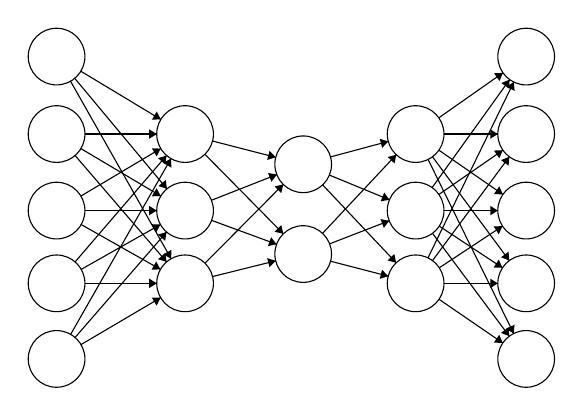
\begin{tikzpicture}[scale=0.12]
\tikzstyle{every node}+=[inner sep=0pt]
\draw [black] (15.7,-15.6) circle (3);
\draw [black] (15.7,-23.8) circle (3);
\draw [black] (15.7,-31.9) circle (3);
\draw [black] (15.7,-39.6) circle (3);
\draw [black] (15.7,-47.6) circle (3);
\draw [black] (29.3,-23.8) circle (3);
\draw [black] (29.3,-31.9) circle (3);
\draw [black] (29.3,-39.6) circle (3);
\draw [black] (41.8,-27) circle (3);
\draw [black] (41.8,-36.5) circle (3);
\draw [black] (53.7,-23.8) circle (3);
\draw [black] (53.7,-31.9) circle (3);
\draw [black] (53.7,-39.6) circle (3);
\draw [black] (65.4,-15.6) circle (3);
\draw [black] (65.4,-23.8) circle (3);
\draw [black] (65.4,-31.9) circle (3);
\draw [black] (65.4,-39.6) circle (3);
\draw [black] (65.4,-47.6) circle (3);
\draw [black] (18.27,-17.15) -- (26.73,-22.25);
\fill [black] (26.73,-22.25) -- (26.3,-21.41) -- (25.79,-22.27);
\draw [black] (17.62,-17.9) -- (27.38,-29.6);
\fill [black] (27.38,-29.6) -- (27.25,-28.66) -- (26.48,-29.3);
\draw [black] (17.18,-18.21) -- (27.82,-36.99);
\fill [black] (27.82,-36.99) -- (27.86,-36.05) -- (26.99,-36.54);
\draw [black] (18.7,-23.8) -- (26.3,-23.8);
\fill [black] (26.3,-23.8) -- (25.5,-23.3) -- (25.5,-24.3);
\draw [black] (18.28,-25.34) -- (26.72,-30.36);
\fill [black] (26.72,-30.36) -- (26.29,-29.53) -- (25.78,-30.39);
\draw [black] (17.66,-26.07) -- (27.34,-37.33);
\fill [black] (27.34,-37.33) -- (27.2,-36.39) -- (26.44,-37.05);
\draw [black] (18.28,-30.36) -- (26.72,-25.34);
\fill [black] (26.72,-25.34) -- (25.78,-25.31) -- (26.29,-26.17);
\draw [black] (18.7,-31.9) -- (26.3,-31.9);
\fill [black] (26.3,-31.9) -- (25.5,-31.4) -- (25.5,-32.4);
\draw [black] (18.31,-33.38) -- (26.69,-38.12);
\fill [black] (26.69,-38.12) -- (26.24,-37.29) -- (25.75,-38.16);
\draw [black] (17.66,-37.33) -- (27.34,-26.07);
\fill [black] (27.34,-26.07) -- (26.44,-26.35) -- (27.2,-27.01);
\draw [black] (18.31,-38.12) -- (26.69,-33.38);
\fill [black] (26.69,-33.38) -- (25.75,-33.34) -- (26.24,-34.21);
\draw [black] (18.7,-39.6) -- (26.3,-39.6);
\fill [black] (26.3,-39.6) -- (25.5,-39.1) -- (25.5,-40.1);
\draw [black] (17.19,-45) -- (27.81,-26.4);
\fill [black] (27.81,-26.4) -- (26.98,-26.85) -- (27.85,-27.35);
\draw [black] (17.66,-45.33) -- (27.34,-34.17);
\fill [black] (27.34,-34.17) -- (26.43,-34.44) -- (27.19,-35.1);
\draw [black] (18.29,-46.08) -- (26.71,-41.12);
\fill [black] (26.71,-41.12) -- (25.77,-41.1) -- (26.28,-41.96);
\draw [black] (32.21,-24.54) -- (38.89,-26.26);
\fill [black] (38.89,-26.26) -- (38.24,-25.57) -- (37.99,-26.54);
\draw [black] (32.09,-30.81) -- (39.01,-28.09);
\fill [black] (39.01,-28.09) -- (38.08,-27.92) -- (38.44,-28.85);
\draw [black] (31.41,-37.47) -- (39.69,-29.13);
\fill [black] (39.69,-29.13) -- (38.77,-29.35) -- (39.48,-30.05);
\draw [black] (31.4,-25.94) -- (39.7,-34.36);
\fill [black] (39.7,-34.36) -- (39.49,-33.44) -- (38.78,-34.14);
\draw [black] (32.12,-32.94) -- (38.98,-35.46);
\fill [black] (38.98,-35.46) -- (38.41,-34.72) -- (38.06,-35.66);
\draw [black] (32.21,-38.88) -- (38.89,-37.22);
\fill [black] (38.89,-37.22) -- (37.99,-36.93) -- (38.23,-37.9);
\draw [black] (44.7,-37.26) -- (50.8,-38.84);
\fill [black] (50.8,-38.84) -- (50.15,-38.16) -- (49.9,-39.13);
\draw [black] (44.6,-35.42) -- (50.9,-32.98);
\fill [black] (50.9,-32.98) -- (49.98,-32.8) -- (50.34,-33.74);
\draw [black] (43.85,-34.31) -- (51.65,-25.99);
\fill [black] (51.65,-25.99) -- (50.74,-26.23) -- (51.47,-26.91);
\draw [black] (44.7,-26.22) -- (50.8,-24.58);
\fill [black] (50.8,-24.58) -- (49.9,-24.3) -- (50.16,-25.27);
\draw [black] (44.57,-28.14) -- (50.93,-30.76);
\fill [black] (50.93,-30.76) -- (50.38,-29.99) -- (50,-30.92);
\draw [black] (43.86,-29.18) -- (51.64,-37.42);
\fill [black] (51.64,-37.42) -- (51.45,-36.49) -- (50.73,-37.18);
\draw [black] (56.16,-22.08) -- (62.94,-17.32);
\fill [black] (62.94,-17.32) -- (62,-17.37) -- (62.58,-18.19);
\draw [black] (56.7,-23.8) -- (62.4,-23.8);
\fill [black] (62.4,-23.8) -- (61.6,-23.3) -- (61.6,-24.3);
\draw [black] (56.17,-25.51) -- (62.93,-30.19);
\fill [black] (62.93,-30.19) -- (62.56,-29.33) -- (61.99,-30.15);
\draw [black] (56.21,-33.55) -- (62.89,-37.95);
\fill [black] (62.89,-37.95) -- (62.5,-37.09) -- (61.95,-37.93);
\draw [black] (55.49,-26.21) -- (63.61,-37.19);
\fill [black] (63.61,-37.19) -- (63.54,-36.25) -- (62.74,-36.84);
\draw [black] (55.02,-26.49) -- (64.08,-44.91);
\fill [black] (64.08,-44.91) -- (64.17,-43.97) -- (63.27,-44.41);
\draw [black] (55.45,-29.46) -- (63.65,-18.04);
\fill [black] (63.65,-18.04) -- (62.78,-18.4) -- (63.59,-18.98);
\draw [black] (56.17,-30.19) -- (62.93,-25.51);
\fill [black] (62.93,-25.51) -- (61.99,-25.55) -- (62.56,-26.37);
\draw [black] (56.7,-31.9) -- (62.4,-31.9);
\fill [black] (62.4,-31.9) -- (61.6,-31.4) -- (61.6,-32.4);
\draw [black] (55.49,-34.31) -- (63.61,-45.19);
\fill [black] (63.61,-45.19) -- (63.53,-44.25) -- (62.73,-44.85);
\draw [black] (55.01,-36.9) -- (64.09,-18.3);
\fill [black] (64.09,-18.3) -- (63.29,-18.8) -- (64.18,-19.23);
\draw [black] (55.49,-37.19) -- (63.61,-26.21);
\fill [black] (63.61,-26.21) -- (62.74,-26.56) -- (63.54,-27.15);
\draw [black] (56.21,-37.95) -- (62.89,-33.55);
\fill [black] (62.89,-33.55) -- (61.95,-33.57) -- (62.5,-34.41);
\draw [black] (56.7,-39.6) -- (62.4,-39.6);
\fill [black] (62.4,-39.6) -- (61.6,-39.1) -- (61.6,-40.1);
\draw [black] (56.18,-41.29) -- (62.92,-45.91);
\fill [black] (62.92,-45.91) -- (62.55,-45.04) -- (61.98,-45.87);
\end{tikzpicture}
 }
  \caption{A possible neural architecture for an AE with a 2-variable encoding layer.}
  \label{p2fig:ae-example}
\end{marginfigure}

The different aspects that lead an AE to a specific transformation are its neural architecture, which determines the type of input and the size of the encoding; the cost and activation functions, which can be defined and regularized in order to induce some desired properties, and parameters of the training process, such as the optimization algorithm or the number of times the data is feeded to the network.


\subsection{Variants}

An interesting advantage of AEs is their versatility: one can obtain encodings with certain properties if the adequate regularizations are chosen. There exist many AE variants in the literature \sidecite{charte2017}, the most common ones centered in how to control the behavior of the transformation while allowing for faithful reconstructions. The following are the most relevant ones:

\begin{itemize}
\item Sparse: induces a low number of activations in average in the encoding layer.
\item Contractive: attempts to preserve the local structure of the original space, thus searching for coordinates in a lower-dimensional manifold.
\item Denoising: is able to remove noise introduced in input examples.
\item Robust: is less sensitive to noise in instances due to a different loss function.
\item Variational: extracts a generative model from the data and is able to produce new, unseen instances.
\item Adversarial: trains in an adversarial manner with the aim of forcing the encoding to follow a given distribution.
\item Convolutional and LSTM-based: are composed of other types of units and layers in order to accomodate bidimensional and sequential data, respectively.
\end{itemize}

%Give the formulations of problems to be solved by the software/toolbox.

%Introduce the background and related work in literature (cite or list algorithms used, other software etc.).

\section{Software Framework }
\label{p2sec.framework}

In this section we elaborate on the internal structure of the developed software and its functionality.

\subsection{Software Architecture}
\label{p2sec.architecture}

% Give a short overview of the overall software architecture.

The object system utilized in \texttt{ruta} is S3, a minimal object orientation from the R language based on generic functions. The software is developed around several classes which have certain applicable methods:

  \begin{itemize}
  \item \texttt{ruta\_autoencoder}: represents a parametrized AE learner. It can be trained and can perform several post-train tasks, such as data encoding and reconstruction.
  \item \texttt{ruta\_network}: defines neural network structures by layers. Networks can be concatenated to produce a longer one.
  \item \texttt{ruta\_loss}: represents the loss function to be optimized by the learner. It is either a wrapper over a loss function from Keras, or a built-in loss function such as correntropy.
  \item \texttt{ruta\_noise}: represents a type of noise which can be applied to input data. Several of these are provided within the package for convenience.
  \end{itemize}


  
\subsection{Software Functionalities}
\label{p2sec.functionality}

The main functionalities of package \texttt{ruta} are as follows:

\begin{itemize}
  \item Define and customize diverse aspects of an AE model.
\item Train AE variants according to the desired objective function.
\item Encode and reconstruct input data with a trained model.
\item Evaluate a trained model according to several metrics which account for quality of reconstruction.
\item Sample generative models created by variational AEs.
  \item Generate corrupted data with different types of noise.
\end{itemize}

The programming interface provided by the package gives several ways to access this set of functionalities, according to the desired level of customization and difficulty:

\begin{itemize}
\item Directly train an AE and compress a database via function \texttt{autoencode}.
\item Define a basic AE simply by enumerating the dimensions of its layers in a vector, e.g. \texttt{autoencoder(c(32, 6))}.
  \item Define each layer composing the neural architecture by means of functions \texttt{input}, \texttt{dense}, {\texttt{conv},} \texttt{output}, etc., then construct an AE with possibly one or more variant properties.
\end{itemize}

The following AE types can be used: basic, sparse, contractive, denoising, robust, variational {and convolutional (via the included \texttt{conv} layers)}. Some of them may be combined by means of the \texttt{make} family of functions, e.g. \texttt{make\_sparse}. They are extensively documented within the package and in the online documentation\footnote{\url{https://ruta.software}}.

%\subsection{Sample code snippets analysis (optional)}
%\label{p2sec.sample}

\subsection{Implementation Details}
\label{p2sec.implementation}

Since \texttt{ruta} is implemented on top of Tensorflow and Keras, it can run on computing devices such as GPUs. In order for them to be used, the correct Tensorflow version with CUDA support will need to be installed. Several issues can arise during the installation and first use, which have been documented in the troubleshooting section of the online documentation.

Few other software pieces provide the necessary functionality to build custom AEs. Among them we can find H2O \sidecite{h2o}, with its \texttt{h2o.deeplearning} function which includes an \texttt{autoencoder} option; package \texttt{autoencoder} for R \sidecite{Rautoencoder}, and library \texttt{yadlt} for Python. These focus on just one or two AE variants and provide less customizability than AEs defined in \texttt{ruta}. For further options one needs to resort to Deep Learning frameworks, which require a much higher programming effort in order to define AE models.

%Implementation details. Empirical results. Conduct empirical studies and provide results. Compare with state-of-the-art software if any, kindly cite relevant work.

\section{Illustrative Examples}
\label{p2sec.examples}

% As stated before, \texttt{ruta} provides its functionality both with a easy-to-use API and with a more customizable

An easy way to start using \texttt{ruta} is by means of the \texttt{autoencode} function. This will take a dataset and  automatically train a simple AE and produce a codification for it. The function accepts several parameters, from which only the desired dimension is mandatory. Other optional parameters are the type of AE, the activation function in the middle layer and the number of epochs for the training process. The following example uses this function to extract 2 features from the well-known toy dataset Iris:

\lstinputlisting[language=R, firstline=1, lastline=4]{papers/02-ruta/example01.R}

These 2 features can be visualized like in Fig.~\ref{p2fig.iris} in order to represent the model learned by the AE.

\begin{marginfigure}
  \centering
  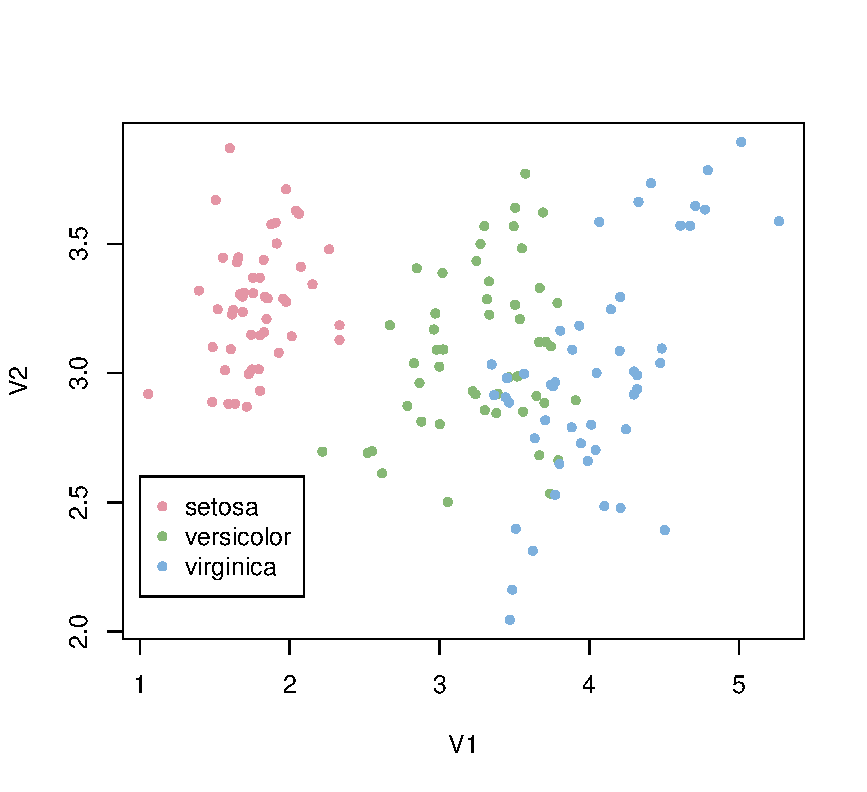
\includegraphics[width=\textwidth]{iris.pdf}
  \caption{Features learned by a basic AE with Iris data.}
  \label{p2fig.iris}
\end{marginfigure}

{The next step in difficulty involves defining a deep autoencoder. To help beginners describe its architecture, \texttt{ruta} provides a conversion from integer vector to neural network architecture in the following manner: \texttt{c(64, 16)} would become a network with an input layer the size of the inputs, a hidden layer with 64 variables, another hidden layer with 16 units for the encoding, the last hidden layer with 64 variables and an output layer the same size of the input one. Thus, the interface allows for simpler code, which can be observed in the following comparison between the code needed to define the same model in \texttt{ruta} and Keras:
}

\lstinputlisting[language=R, firstline=1, lastline=29]{papers/02-ruta/example05.R}

The following example loads a dataset from Keras and normalizes its variables. Afterwards it defines a sparse AE by means of the \texttt{autoencoder\_sparse} function with a 3-variable encoding, trains it and uses it to reconstruct test data. An evaluation is performed according to the mean squared error metric for the same test data.

\lstinputlisting[language=R, firstline=4, lastline=20]{papers/02-ruta/example02.R}

Another task that can be performed by a trained variational AE is generation of new instances. In this case, we load the MNIST dataset of handwritten digits and learn 10 features which can be sampled via the \texttt{generate} function. Instances can also be generated by interpolating encodings from existing instances and decoding those interpolations, as Fig.~\ref{p2fig.variational} shows.

\lstinputlisting[language=R, firstline=4, lastline=22]{papers/02-ruta/example03.R}


\begin{figure}[ht]
  \centering
  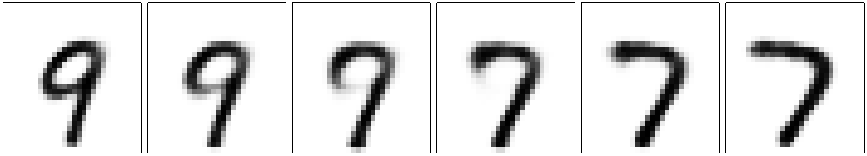
\includegraphics[width=0.8\columnwidth]{variational_97.pdf}
  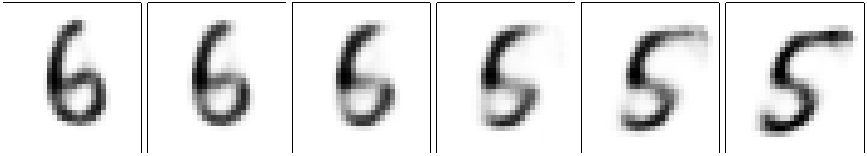
\includegraphics[width=0.8\columnwidth]{variational_65.pdf}
  \caption{Instances generated when interpolating between test samples in a variational AE trained with MNIST data.}
  \label{p2fig.variational}
\end{figure}

{The generic AE templates provided within the package may not always be adaptable enough for some problems. Thus, in order to provide detailed control over the model for more advanced users with some knowledge of Keras, \texttt{ruta} can convert its AE objects into a list of Keras models. This list contains three models: one for the encoder, another one for the decoder and one for the full AE. It can be accessed by setting the input shape in the Ruta object and calling the \texttt{to\_keras} method:}

\lstinputlisting[language=R, firstline=4, lastline=7]{papers/02-ruta/example06.R}

Individual examples for each AE type are provided in the online documentation, as well as detailed instructions on how to build more customized neural architectures.

%\lstinputlisting[language=R]{example_paper.R}

%Provide at least one illustrative example to demonstrate the major functions.

%Optional: you may include one explanatory video that will appear next to your article, in the right hand side panel. (Please upload any video as a single supplementary file with your article. Only one MP4 formatted, with 50MB maximum size, video is possible per article. Recommended video dimensions are 640 $\times$ 480 at a maximum of 30 frames/second. Prior to submission please test and validate your .mp4 file at $ http://elsevier-apps.sciverse.com/GadgetVideoPodcastPlayerWeb/verification$. This tool will display your video exactly in the same way as it will appear on ScienceDirect.).


\section{Conclusions}
\label{p2sec.conclusions}

% Set out the conclusion of this original software publication.

In this paper, we have presented a novel software piece focused in the construction of AEs, the \texttt{ruta} package for R. As opposed to most software developed on this topic, \texttt{ruta} implements several well-known AE variants and can handle different datasets. The software is implemented on top of Tensorflow and Keras in order to provide good performance{, but abstracts many common aspects of AEs in order to provide an easy-to-use interface, accessible to R users with or without a programming background}.

We have provided examples on how trained AEs can perform several tasks such as encoding and reconstruction of new data, as well as evaluation and even instance generation. {When users need more control over the automatic generation of AE architectures, the package allows to extract the associated Keras models so as not to hinder their customization.}

{Since its publication on CRAN in May 2018 to the end of the year, \texttt{ruta} has received more than a thousand downloads from the RStudio CRAN mirror. Fig. \ref{p2fig.downloads} shows the amount of downloads since the day of publication.}

\begin{marginfigure}
  \centering
  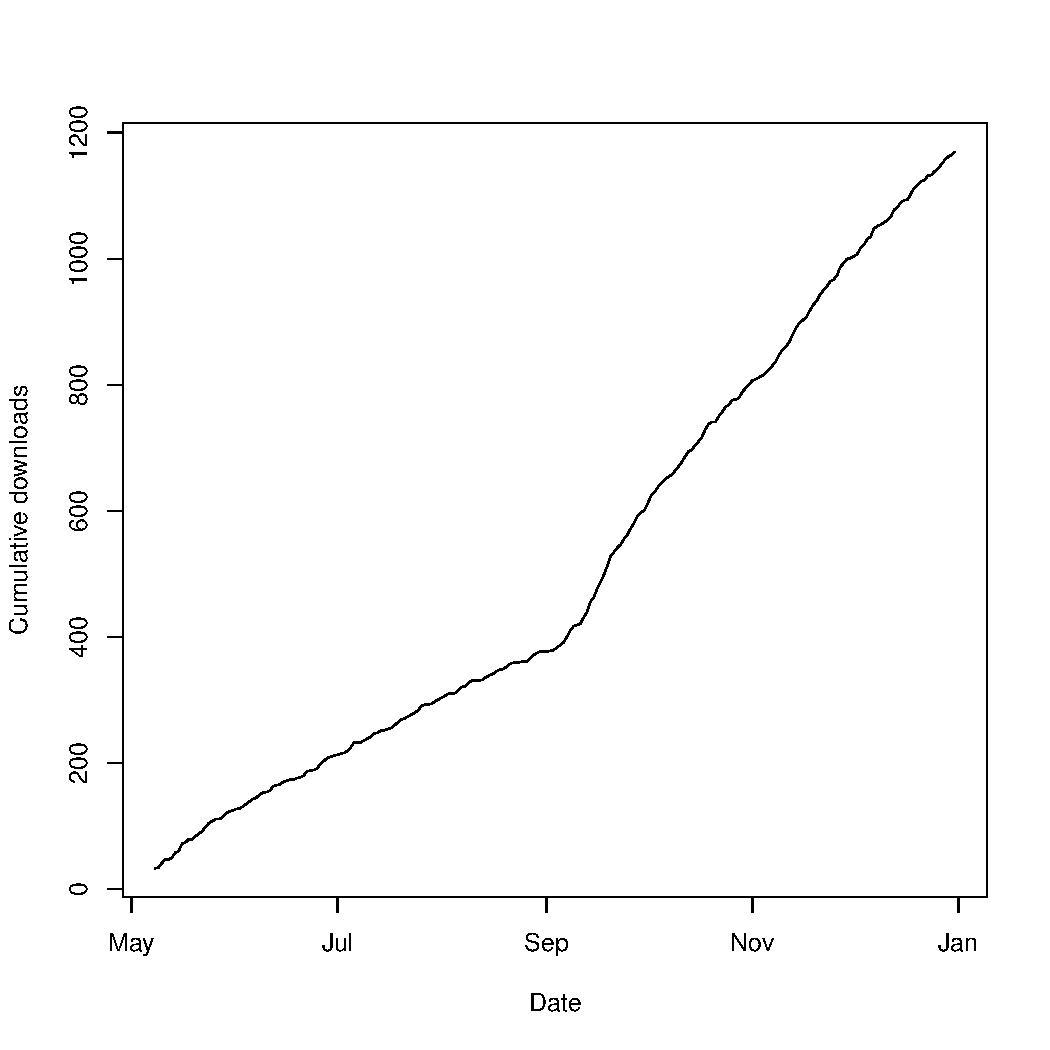
\includegraphics[width=\textwidth]{ruta_downloads.pdf}
  \caption{\label{p2fig.downloads}Cumulative downloads since \texttt{ruta} was published.}
\end{marginfigure}

Some supplementary software packages have already been planned. These include a package dedicated to visualizing the behavior of AEs, from their training process to the learned model, and a web-based user interface with the aim of providing easier access to these neural architectures.

% DONE No extensiones sino paquetes complementarios para el futuro, en un párrafo aparte, herramientas de visualización e interfaz GUI. 
% DONE Ref. 1 Citar libro y no el capítulo de introducción - ari-dasci - youtube
% revisar formato (overfulls)

\section*{Acknowledgements}
\label{p2sec.acknowledgements}

This work was partially funded by the grant Iniciaci{\'o}n a la Investigaci{\'o}n para Alumnos de M{\'a}ster of the University of Granada, project TIN2015-68854-R (FEDER Founds) of the Spanish Ministry of Economy and Competitiveness and project BigDaP-TOOLS - Ayudas
Fundaci{\'o}n BBVA a Equipos de Investigaci{\'o}n  Cient{\'i}fica
2016.

%% The Appendices part is started with the command \appendix;
%% appendix sections are then done as normal sections
%% \appendix

%% \section{}
%% \label{p2}

%% References: At least 5 are required 
%% If you have bibdatabase file and want bibtex to generate the
%% bibitems, please use
%%
%\bibliographystyle{elsarticle-num} 
%\bibliography{references}

%% else use the following coding to input the bibitems directly in the
%% TeX file.
% \begin{widepar}\leavevmode
%   \section*{References}
%   \printbibliography[heading=none]
% \begin{thebibliography}{10}
% \expandafter\ifx\csname url\endcsname\relax
%   \def\url#1{\texttt{#1}}\fi
% \expandafter\ifx\csname urlprefix\endcsname\relax\def\urlprefix{URL }\fi
% \expandafter\ifx\csname href\endcsname\relax
%   \def\href#1#2{#2} \def\path#1{#1}\fi

% \bibitem{PCABook}
% I.~T. Jolliffe, Introduction, in: Principal component analysis, Springer, 1986,
%   pp. 1--7.
% \newblock \href {http://dx.doi.org/10.1007/978-1-4757-1904-8}
%   {\path{doi:10.1007/978-1-4757-1904-8}}.

% \bibitem{MDS}
% W.~S. Torgerson, Multidimensional scaling: I. theory and method, Psychometrika
%   17~(4) (1952) 401--419.
% \newblock \href {http://dx.doi.org/10.1007/BF02288916}
%   {\path{doi:10.1007/BF02288916}}.

% \bibitem{Isomap}
% J.~B. Tenenbaum, V.~De~Silva, J.~C. Langford, A global geometric framework for
%   nonlinear dimensionality reduction, science 290~(5500) (2000) 2319--2323.
% \newblock \href {http://dx.doi.org/10.1126/science.290.5500.2319}
%   {\path{doi:10.1126/science.290.5500.2319}}.

% \bibitem{LLE}
% S.~T. Roweis, L.~K. Saul, Nonlinear dimensionality reduction by locally linear
%   embedding, science 290~(5500) (2000) 2323--2326.
% \newblock \href {http://dx.doi.org/10.1126/science.290.5500.2323}
%   {\path{doi:10.1126/science.290.5500.2323}}.

% \bibitem{tSNE}
% L.~v.~d. Maaten, G.~Hinton, Visualizing data using t-sne, Journal of machine
%   learning research 9~(Nov) (2008) 2579--2605.

% \bibitem{RBM}
% I.~Goodfellow, Y.~Bengio, A.~Courville, Deep Learning, MIT Press, 2016, Ch.
%   Deep generative models, pp. 651--716, \url{http://www.deeplearningbook.org}.

% \bibitem{hinton_reducing_2006}
% G.~E. Hinton,
%   \href{http://www.sciencemag.org/cgi/doi/10.1126/science.1127647}{Reducing the
%   dimensionality of data with neural networks}, Science 313~(5786) (2006)
%   504--507.
% \newblock \href {http://dx.doi.org/10.1126/science.1127647}
%   {\path{doi:10.1126/science.1127647}}.
% \newline\urlprefix\url{http://www.sciencemag.org/cgi/doi/10.1126/science.1127647}

% \bibitem{Keras}
% F.~Chollet, et~al., Keras, \url{https://github.com/fchollet/keras} (2015).

% \bibitem{Tensorflow}
% M.~Abadi, P.~Barham, J.~Chen, Z.~Chen, A.~Davis, et~al., Tensorflow: A system
%   for large-scale machine learning, in: Proceedings of the 12th USENIX
%   Conference on Operating Systems Design and Implementation, OSDI'16, USENIX
%   Association, Berkeley, CA, USA, 2016, pp. 265--283.

% \bibitem{charte2017}
% D.~Charte, F.~Charte, S.~Garc{\'i}a, M.~J. del Jesus, F.~Herrera, A practical
%   tutorial on autoencoders for nonlinear feature fusion: Taxonomy, models,
%   software and guidelines, Information Fusion 44 (2018) 78 -- 96.
% \newblock \href {http://dx.doi.org/10.1016/j.inffus.2017.12.007}
%   {\path{doi:10.1016/j.inffus.2017.12.007}}.

% \bibitem{h2o}
% E.~LeDell, N.~Gill, S.~Aiello, A.~Fu, A.~Candel, C.~Click, T.~Kraljevic,
%   T.~Nykodym, P.~Aboyoun, M.~Kurka, M.~Malohlava,
%   \href{https://CRAN.R-project.org/package=h2o}{h2o: R Interface for 'H2O'}, r
%   package version 3.20.0.2 (2018).
% \newline\urlprefix\url{https://CRAN.R-project.org/package=h2o}

% \bibitem{Rautoencoder}
% E.~Dubossarsky, Y.~Tyshetskiy,
%   \href{https://CRAN.R-project.org/package=autoencoder}{autoencoder: Sparse
%   Autoencoder for Automatic Learning of Representative Features from Unlabeled
%   Data}, r package version 1.1 (2015).
% \newline\urlprefix\url{https://CRAN.R-project.org/package=autoencoder}

% \end{thebibliography}
% \end{widepar}

%\begin{thebibliography}{00}

%% \bibitem{label}
%% Text of bibliographic item

%\bibitem{}

%\end{thebibliography}

% \clearpage
% \section*{Required Metadata}

% \section*{Current executable software version}

% Table~\ref{p2tbl.exe}

% \begin{table*}[!h]
% \begin{tabular}{|l|p{6.5cm}|p{6.5cm}|}
% \hline
% \textbf{Nr.} & \textbf{(executable) Software metadata description} & \textbf{Please fill in this column} \\
% \hline
% S1 & Current software version & 1.{1.0} \\
% \hline
% S2 & Permanent link to executables of this version  & {\url{https://github.com/fdavidcl/ruta/releases/tag/1.1.0}} \\
% \hline
% S3 & Legal Software License & GPL-3.0 \\
% \hline
% S4 & Computing platform/Operating System & Linux, OS X, Microsoft Windows \\
% \hline
% S5 & Installation requirements \& dependencies & Python, R, Tensorflow, Keras \\
% \hline
% S6 & If available, link to user manual - if formally published include a reference to the publication in the reference list & \url{https://ruta.software/reference/} \\
% \hline
% S7 & Support email for questions & fdavidcl@ugr.es \\
% \hline
% \end{tabular}
% \caption{Software metadata}
% \label{p2tbl.exe} 
% \end{table*}

% \section*{Current code version}

% Table~\ref{p2tbl.code}

% \begin{table*}[!h]
% \begin{tabular}{|l|p{6.5cm}|p{6.5cm}|}
% \hline
% \textbf{Nr.} & \textbf{Code metadata description} & \textbf{Please fill in this column} \\
% \hline
% C1 & Current code version & 1.{1.0} \\
% \hline
% C2 & Permanent link to code/repository used of this code version & {\url{https://github.com/fdavidcl/ruta/tree/1.1.0/}} \\
% \hline
% C3 & Legal Code License   & GPL-3.0 \\
% \hline
% C4 & Code versioning system used & git \\
% \hline
% C5 & Software code languages, tools, and services used & R \\
% \hline
% C6 & Compilation requirements, operating environments \& dependencies & R developer tools \\
% \hline
% C7 & If available Link to developer documentation/manual & \url{https://ruta.software/reference/} \\
% \hline
% C8 & Support email for questions & fdavidcl@ugr.es \\
% \hline
% \end{tabular}
% \caption{Code metadata}
% \label{p2tbl.code} 
% \end{table*}

% \end{document}
% \endinput
%%
%% End of file `OSP_Latex_template.tex'.
